
                \begin{figure}
                    \centering
                    \begin{tikzpicture}
                        \pgfplotsset{%
                            width=1\textwidth,
                            height=0.4\textheight
                        }
                        \begin{axis}[
                            xlabel={Runs since restart},
                            ylabel={Average dynamic energy (watt)},
                            ymin=0,ymax=70,
                        ]
                        
                            \addplot [mark=none, densely dashed, red]  coordinates {
                            (1, 19.73790788402818)(2, 18.081814688529462)(3, 17.692188302923622)(4, 17.84392707638979)(5, 17.71410661329038)
                            };
                            \addlegendentry{WRK - IPG}
                            
                            \addplot [mark=none, densely dashed, blue]  coordinates {
                            (1, 18.454259900938062)(2, 18.048697213767806)(3, 18.10548096477223)(4, 17.969210775235464)(5, 17.636008024440272)
                            };
                            \addlegendentry{WRK - LHM}
                            
                            \addplot [mark=none, densely dashed, cyan]  coordinates {
                            (1, 14.635944924787315)(2, 13.472357009871592)(3, 15.041412497265261)(4, 13.873635272363714)(5, 13.4386067999369)
                            };
                            \addlegendentry{WRK - CLAMP (win)}
                            
                            \addplot [mark=none, densely dashed, orange]  coordinates {
                            (1, 27.775549459481347)(2, 27.607037990852078)(4, 27.71887559807309)(5, 27.639561703505834)(6, 27.821597313428533)(7, 27.699217730731213)(8, 27.730583141470966)(9, 27.730023612779036)(10, 27.682323844341518)(11, 27.717899682503408)(12, 27.76909495833)(13, 27.680102215812063)(15, 27.68997859939777)(16, 27.564945729091384)(17, 27.66663245749706)(18, 27.70809745521057)(19, 27.629976572835794)(20, 27.65658687334915)(21, 27.700629739969727)(22, 27.7419317570708)(23, 27.713621741410954)(24, 27.55267691503215)(25, 27.604983801184957)(26, 27.67168457271743)(27, 27.654134296304726)(28, 27.683653809533254)(29, 27.50143600522992)
                            };
                            \addlegendentry{WRK - RAPL}
                            
                            \addplot [mark=none, densely dashed, black]  coordinates {
                            (1, 28.00573049378532)(2, 28.108132807005276)(4, 27.601944495704842)(6, 27.920780176446357)(7, 27.565981694585673)(8, 28.146591542653383)(9, 27.805089553954318)(10, 28.185076354740602)(11, 28.144293617255244)(12, 27.790671289437952)(13, 28.189224826469214)(14, 27.845855364244215)(15, 27.707543288275232)(16, 28.180312152600152)(17, 27.31880982234972)(18, 27.756109775084298)(20, 27.505347287108208)(21, 27.486716264446628)(23, 27.46710083147819)(24, 27.433812384843776)(26, 27.29175082143304)(28, 27.899217216442153)(29, 28.040066875747186)
                            };
                            \addlegendentry{WRK - CLAMP (lin)}
                            
                        \end{axis}
                    \end{tikzpicture} 
                \caption{A graph illustrating the energy consumption of Cores for test case Nbody with regards to how long ago the DUT was restarted, experiment \#2, (without outliers)} \label{fig:Nbody_Cores_iteration_exp2}
                \end{figure}
                